\section{Introduction}

Enterprise Resource Planning (ERP) systems have marked a transformative shift in the IT industry since the mid-1990s. 
This transformation is characterized by three key aspects: 
\begin{enumerate}
    \item It has become a global phenomenon.
    \item It has shifted the focus from custom-built software solutions to packaged systems supported by consulting services.
    \item It has unified and integrated three critical portfolios into a cohesive framework.
\end{enumerate}
\begin{figure}[H]
    \centering
    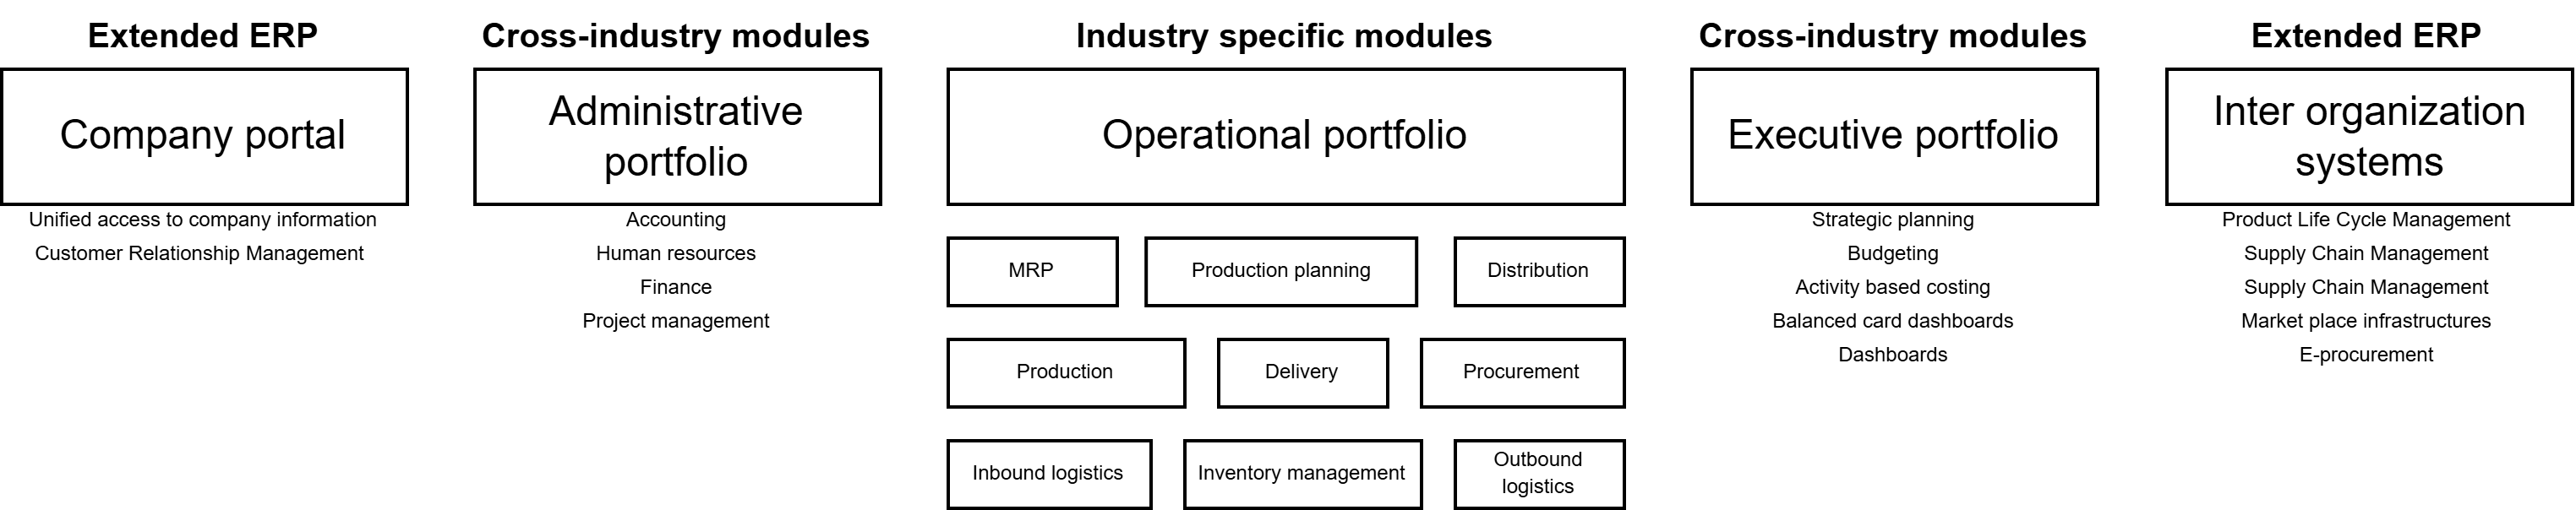
\includegraphics[width=1\linewidth]{images/bis1.png}
    \caption{ERP architecture}
\end{figure}
\noindent A fundamental distinction exists between two types of ERP modules:
\begin{itemize}
    \item \textit{Core ERP}: these modules support internal processes within an organization. 
        They encompass administrative functions, vertical operational tasks, and executive decision-making tools.
    \item \textit{Extended ERP}: these modules facilitate interactions with external entities.
        They include Customer Relationship Management (CRM), Supply Chain Management (SCM), e-procurement platforms, and online marketplaces.
\end{itemize}

\paragraph*{Principles}
ERP systems are built on three foundational principles:
\begin{enumerate}
    \item \textit{Information integration}: ERP systems aim to unify data across all levels of an organization. 
        This includes vertical, horizontal and conceptual consistencies through a single, integrated data model that eliminates silos and promotes unified insights.
    \item \textit{Extension and modularity}: ERP systems are designed to be functionally comprehensive while offering flexibility through modular components:
        \begin{itemize}
            \item \textit{One-stop shopping}: a single supplier provides all modules, ensuring compatibility and streamlined implementation.
            \item \textit{Best-of-breed}: organizations can choose modules from multiple suppliers, allowing for tailored solutions but potentially increasing integration complexity.
        \end{itemize}
    \item \textit{Process prescriptiveness}: ERP systems embed predefined process logic, which often necessitates organizational change. 
        While this prescriptiveness offers advantages, it also presents challenges, including potential constraints on diversification and competitiveness.
\end{enumerate}
\noindent No single ERP provider can deliver all functionalities required across every industry. 
Instead, niche players often specialize in offering industry-specific solutions tailored to unique business needs. 
This creates opportunities for system integration, allowing companies to combine software from multiple vendors to create a comprehensive and customized solution.

Small and medium-sized businesses typically opt for more flexible and cost-effective options, such as simplified ERP packages (often referred to as ERP Light), Software-as-a-Service (SaaS), or Cloud-based solutions. 